\begin{frame}{Введение}
  \begin{itemize}
    \item Введение
    \item Возможности
    \item Обзор архитектуры
    \item Примеры, примеры, примеры 
    \item Нюансы использования
    \item NFSTrace: Пример
  \end{itemize}
\end{frame}

\begin{frame}{Введение}
  \begin{center}
    \Large Зачем все это?
  \end{center}
\end{frame}

\begin{frame}{Перед тем как наченм}
  \begin{block}{Sir Charles Dilke, 1892 г.}
    Существует три вида лжи: ложь, наглая ложь и статистика.
  \end{block}
\end{frame}

\begin{frame}{Возможности}
  \begin{itemize}
    \item Как часто выполняется каждая строчка кода\footnote{покрытие по функциям, веткам исполнения}
    \item Какие именно строки кода были выполнены
    \item Сколько времени заняло выполнение каждой секции
  \end{itemize}
\end{frame}

\begin{frame}{Ключи компиляции gcc}
  \begin{itemize}
    \item O0 (компиляция без оптимизации)
    \item Ключ -ftest-coverage (после компиляции: gcno )
    \item Ключ -fprofile-arcs (после запуска:  gcda)
    \item -{}-coverage (2 ключа объединены)
  \end{itemize}
\end{frame}

\begin{frame}{Архитектура: Базовый блок}
    \begin{block}{Базовый блок}
        Последовательность инструкций, имеющая одну точку входа и одну точку выхода.
    \end{block}
\end{frame}

\begin{frame}{Архитектура: gcno файл}
  \begin{itemize}
    \item Файл создается после компиляции
    \item Граф базовых блоков
    \item Маппинг базовых блоков на строки кода
  \end{itemize}
\end{frame}

\begin{frame}{Архитектура: gcda файл}
  \begin{itemize}
      \item Создается после выполнения программы
      \item Создается для каждого объектного файла\footnote{скомпилированного с опцией -fprofile-arcs}
      \item Содержит статистику исполнения программы
  \end{itemize}
\end{frame}


\begin{frame}{Архитектура: gcda файл}
  \begin{center}
    \large Накапливает статистику для каждого запуска!\footnote{Более подробно: gcov-io.h}
  \end{center}
\end{frame}

\begin{frame}{Архитектура: gcov файл}
  \begin{itemize}
      \item gcov [ключи] [SOURCE|OBJ]
      \item На выходе *.gcov файл
      \item Подробная информация об исполнении
  \end{itemize}
\end{frame}

\begin{frame}{gcov: ключи}
  \begin{itemize}
      \item Функциональные для анализа: a, b, c, f, u
      \item Вспомогательные для деплоймента: p, r, f, o, s
      \item Остальные: m, i, d
  \end{itemize}
\end{frame}

\begin{frame}{Нюансы использования}
  \begin{itemize}
      \item Сложный код (несколько инструкций на одной строке)
      \item Макросы
      \item Виртуальные функции/деструкторы (Пример 4)  
  \end{itemize}
\end{frame}

\begin{frame}{Пример 1 (часть 1)}
  \begin{enumerate}
      \item Зайти в директории hello
      \item vi makefile (ключи компиляции)
      \item vi hello.c 
      \item make (появится hello.gcno)
      \item ./hello 1 (появится hello.gcda)
      \item gcov hello.c (появится hello.c.gcov)
      \item vi hello.c.gcov
  \end{enumerate}
\end{frame}

\begin{frame}{Пример 1 (часть 2)}
  \begin{enumerate}
      \item ./hello 1
      \item gcov hello.c (посмотреть что изменилось)
      \item ./hello 2
      \item gcov hello.c
      \item vi hello.c.gcov 
      \item ./hello 3
      \item gcov hello.c (100\%)
  \end{enumerate}
\end{frame}

\begin{frame}{Пример 2 (ветвление)}
  \begin{enumerate}
      \item Удалить 2 if из hello.c
      \item make clean
      \item make
      \item ./hello 1
      \item gcov -b hello.c (branch taken / branch executed)\footnote{Обратить внимание на количесвто branch-ей}
      \item ./hello 2 
      \item gcov -b hello.c (branch taken / branch executed)
  \end{enumerate}
\end{frame}

\begin{frame}{Пример 3 (статистика по функцииям)}
  \begin{enumerate}
      \item Перейти в каталог core
      \item Изучить core.c core.h main.c
      \item make
      \item ./core
      \item gcov -f core (статистика по фукнциям)
      \item Добавить вызов Calc2 в main.c
      \item Посмотреть как изменится статистика
  \end{enumerate}
\end{frame}

\begin{frame}{Пример 4 (виртуальный деструктор)}
  \begin{enumerate}
      \item Перейт в каталог ctor
      \item Изучить makefile (параметр gcov)
      \item Запустить make gcov
      \item Обратить внимание на строку "Taken at least once 50\% of 2"
      \item Объяснить полученый результат\footnote{Дополнительная информация: \url{http://stackoverflow.com/questions/7199360/what-is-the-branch-in-the-destructor-reported-by-gcov}}
  \end{enumerate}
\end{frame}

\begin{frame}{Пример 5 (когда 100\% != все строки кода)}
  \begin{enumerate}
      \item Перейт в каталог hello100 
      \item make 
      \item ./hello100 1 
      \item gcov hello100 
      \item Обратить внимание на строку "Lines executed:100.00\%"
  \end{enumerate}
\end{frame}


\begin{frame}{Пример: NFSTrace}
  \begin{center}
    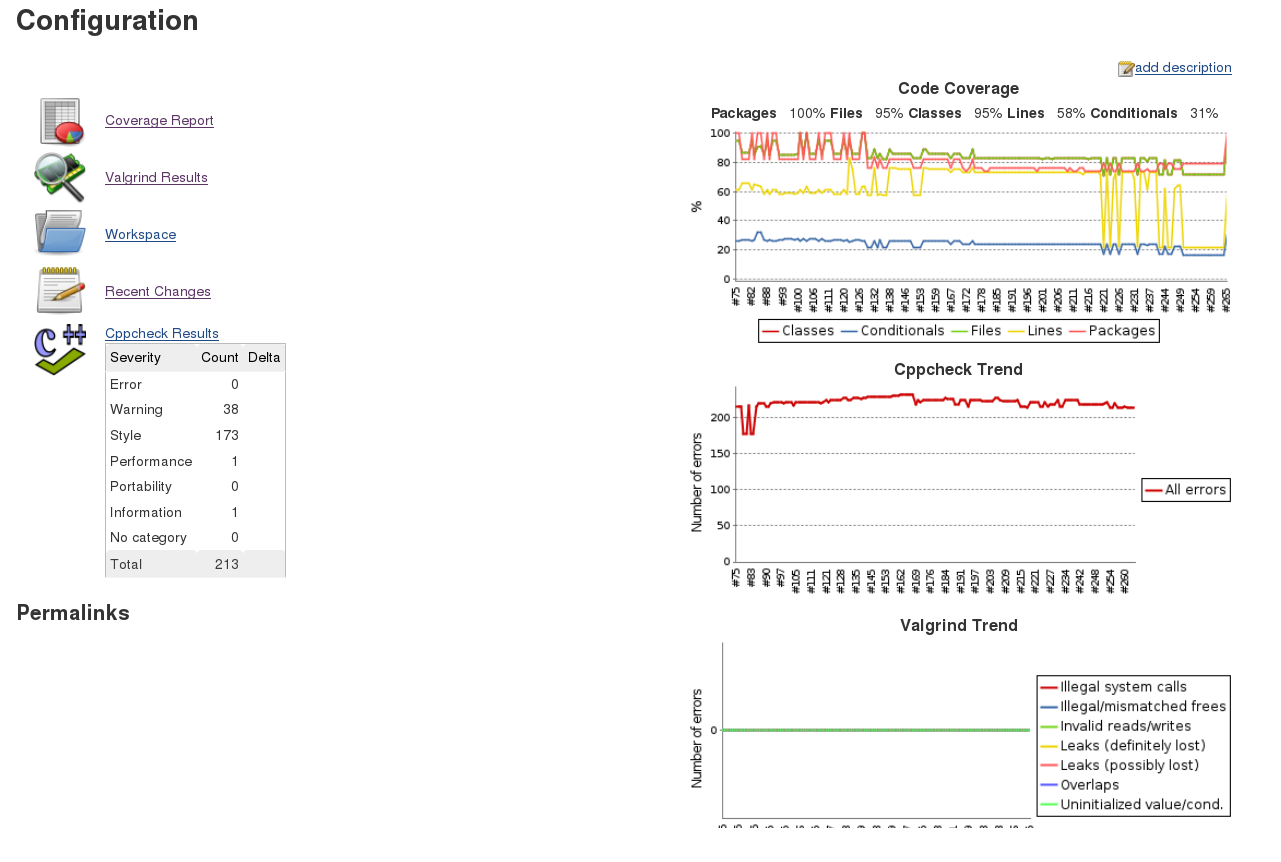
\includegraphics[height=0.9\textheight]{../../slides/profile/nfs-trace-coverage.png}
  \end{center}
\end{frame}

\begin{frame}{Пример: NFSTrace}
  \begin{center}
    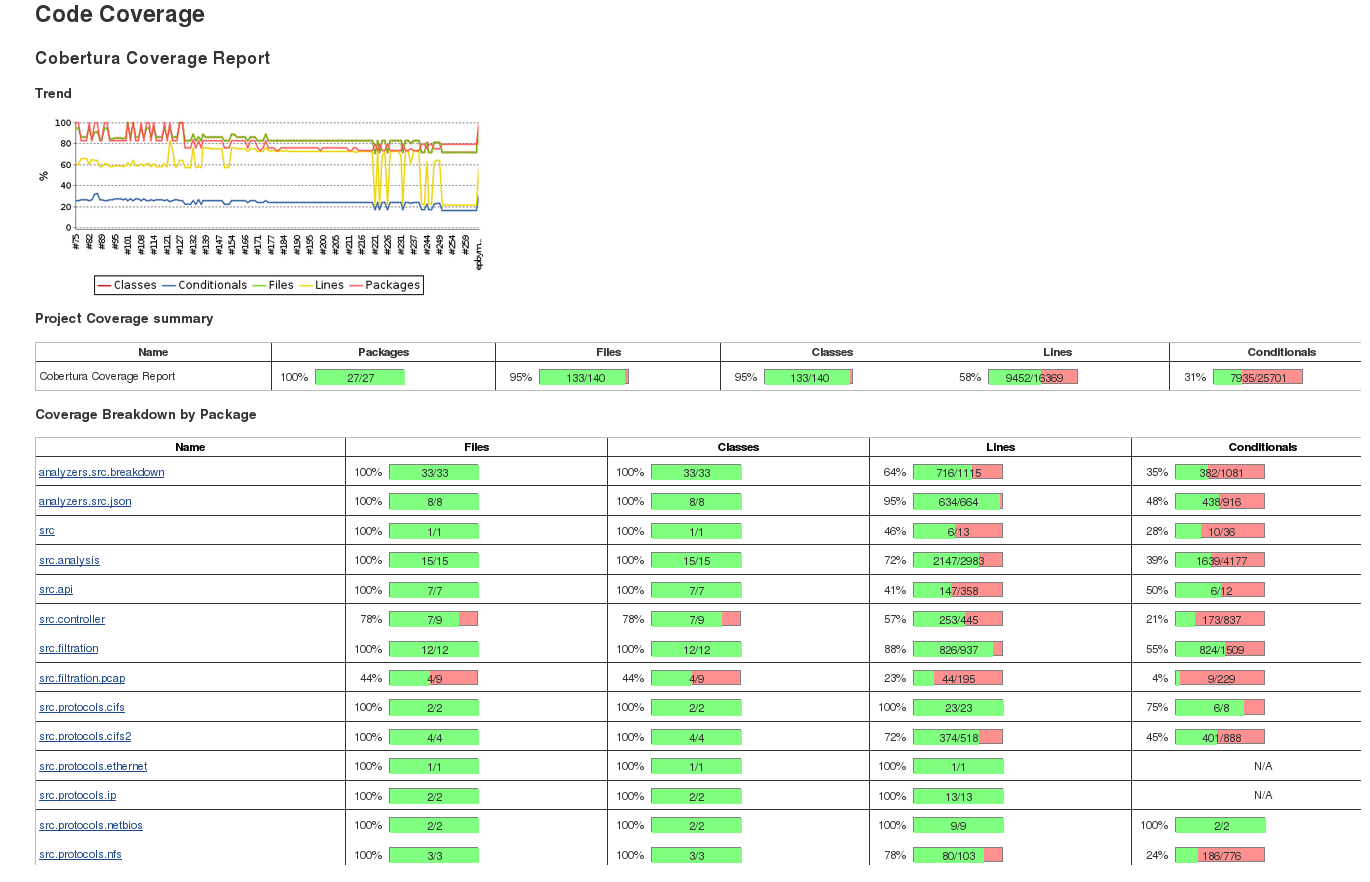
\includegraphics[height=0.9\textheight]{../../slides/profile/nfs-trace-coverage-html.png}
  \end{center}
\end{frame}

